\documentclass[12pt,a4paper]{article}
\usepackage{amsmath,amssymb}
\usepackage{fontspec}
\usepackage{polyglossia}
\setdefaultlanguage{russian}
\setotherlanguage{english}
\setmainfont{Liberation Serif}
\newfontfamily\cyrillicfont{Liberation Serif}
\newfontfamily\logofont{Liberation Sans}
\usepackage[a4paper,left=2cm,right=1.7cm,top=1.8cm,bottom=2cm]{geometry}
\usepackage{array,longtable,multirow,makecell,tabularx}
\usepackage{tikz}
\usetikzlibrary{arrows.meta,patterns,calc}
\usepackage{pgfplots}
\pgfplotsset{compat=1.18}
\usepackage{caption}
\captionsetup{labelsep=endash,justification=centering,font=normalsize}
\usepackage{enumitem}
\setlist[itemize]{label=\textbullet,leftmargin=1.2cm,itemsep=1pt,topsep=3pt}
\usepackage{xcolor}

\setlength{\parindent}{0pt}
\setlength{\parskip}{4pt}
\renewcommand{\arraystretch}{1.25}
\newcolumntype{C}[1]{>{\centering\arraybackslash}m{#1}}
\newcolumntype{L}[1]{>{\raggedright\arraybackslash}m{#1}}

% поле с подчёркиванием (как в бланке)
\let\oldsum\sum
\renewcommand{\sum}{\oldsum\limits}
\newcommand{\fld}[2]{\underline{\makebox[#1][l]{\ #2}}}
% заголовок пункта протокола-отчёта
\newcommand{\punkt}[1]{\par\vspace{14pt}\noindent{\fontsize{14}{17}\selectfont #1}\par\vspace{3pt}}
% ячейка с формулой
\newcommand{\fm}[1]{\vspace{3pt}$\displaystyle #1$\vspace{3pt}}

\pagestyle{plain}

\begin{document}

%======================== ШАПКА ========================
\noindent
\begin{minipage}[c]{0.55\textwidth}
\centering\bfseries
Университет ИТМО\\
Физико-технический мегафакультет\\
Физический факультет
\end{minipage}\hfill
\begin{minipage}[c]{0.4\textwidth}
\centering
\begin{tikzpicture}
  \fill (0,0) rectangle (0.24,1.05);
  \fill (0.36,0) -- (0.62,0) -- (1.06,1.05) -- (0.80,1.05) -- cycle;
  \node[anchor=south west,inner sep=0pt] at (1.02,-0.02)
    {\logofont\bfseries\fontsize{42}{42}\selectfont TMO};
\end{tikzpicture}
\end{minipage}

\vspace{6pt}
\noindent\rule{\textwidth}{0.6pt}

\vspace{-4pt}
\noindent
\begin{tabular}{@{}p{0.5\textwidth}@{\hspace{0.04\textwidth}}p{0.44\textwidth}@{}}
Группа\fld{6.6cm}{ФИЗ ПИИКТ 2.1.1} & К работе допущен\fld{4.3cm}{} \\
Студент\fld{6.4cm}{Бригада 8 (Добкес, Пегушина)} & Работа выполнена\fld{4.2cm}{} \\
Преподаватель\fld{5.25cm}{Сорокина Елена} & Отчет принят\fld{4.9cm}{} \\
\fld{8.1cm}{Константиновна} & \\
\end{tabular}

\vspace{2pt}
\begin{center}
{\fontsize{20}{24}\selectfont\bfseries\addfontfeatures{LetterSpace=8}
Рабочий протокол и отчет по\\[2pt]
лабораторной работе № 1.02\par}
\vspace{4pt}
{\fontsize{17}{21}\selectfont Изучение скольжения тележки\\ по наклонной плоскости\par}
\end{center}
\vspace{-6pt}
\noindent\rule{\textwidth}{0.6pt}

%======================== 1 ========================
\punkt{1. Цель работы.}
\begin{itemize}
  \item Экспериментальная проверка равноускоренности движения тела по наклонной плоскости.
  \item Определение величины ускорения свободного падения.
\end{itemize}

%======================== 2 ========================
\punkt{2. Задачи, решаемые при выполнении работы.}
\begin{itemize}
  \item Измерить зависимость времени движения от пройденного расстояния при движении тела по наклонной плоскости с фиксированным углом наклона.
  \item Измерить зависимость времени прохождения телом фиксированного расстояния от угла наклона плоскости к горизонту.
  \item Исследовать зависимость времени движения от пройденного расстояния при движении тела по наклонной плоскости при фиксированном угле наклона плоскости.
  \item Исследовать зависимость времени прохождения телом фиксированного расстояния от угла наклона рельса к горизонту.
  \item Исследовать зависимость ускорения тела от угла наклона рельса к горизонту.
\end{itemize}

%======================== 3 ========================
\punkt{3. Объект исследования.}
Тележка, скользящая на воздушной подушке по наклонному рельсу (наклонной плоскости). Воздушная подушка, создаваемая насосом, уменьшает трение между тележкой и рельсом; угол наклона рельса к горизонту задаётся числом стандартных пластин, подложенных под левую опору рельса.

%======================== 4 ========================
\punkt{4. Метод экспериментального исследования.}
Метод основан на измерении времени $t_1$, $t_2$ прохождения тележкой оптических ворот $x_1$, $x_2$ и последующем расчёте (методом наименьших квадратов) ускорения тележки $a$ по зависимости $Y = x_2 - x_1$ от $Z = (t_2^2 - t_1^2)/2$, а также ускорения свободного падения $g$ по зависимости $a = A + B\sin\alpha$.

%======================== 5 ========================
\punkt{5. Рабочие формулы и исходные данные.}
Рабочие формулы:

\begin{longtable}{|C{0.7cm}|C{10.9cm}|L{4.3cm}|}
\hline
1 & \fm{x_2 - x_1 = \frac{a}{2}\left(t_2^2 - t_1^2\right)} & Связь перемещения и времени движения при равноускоренном движении из состояния покоя \\ \hline
2 & \fm{a = g\sin\alpha - \frac{F_\text{тр}}{m}} & Ускорение тележки на наклонной плоскости (2-й закон Ньютона) \\ \hline
3 & \fm{Y = x_2 - x_1, \qquad Z = \frac{t_2^2 - t_1^2}{2}} & Величины, связанные линейно: $Y = aZ$ \\ \hline
4 & \fm{\Delta_Y = \sqrt{\left(\Delta_{x_{\text{и}1}}\right)^2 + \left(\Delta_{x_{\text{и}2}}\right)^2} = \sqrt{2}\,\Delta_{x_\text{и}}} & Абсолютная погрешность $Y$ \\ \hline
5 & \fm{\delta_Y = \frac{\Delta_Y}{Y}\cdot 100\,\%} & Относительная погрешность $Y$ \\ \hline
6 & \fm{\Delta_Z = \sqrt{\left(t_1\Delta_{t_{\text{и}1}}\right)^2 + \left(t_2\Delta_{t_{\text{и}2}}\right)^2} = \Delta_{t_\text{и}}\sqrt{t_1^2 + t_2^2}} & Абсолютная погрешность $Z$ \\ \hline
7 & \fm{\delta_Z = \frac{\Delta_Z}{Z}\cdot 100\,\%} & Относительная погрешность $Z$ \\ \hline
\multicolumn{3}{|C{16.6cm}|}{Метод наименьших квадратов для зависимости $Y = aZ$ (прямая через начало координат), $n = 5$} \\ \hline
8 & \fm{a = \frac{\sum_{i=1}^{n} Z_i Y_i}{\sum_{i=1}^{n} Z_i^2}} & Ускорение тележки (угловой коэффициент) \\ \hline
9 & \fm{S_a = \sqrt{\frac{\sum_{i=1}^{n}\left(Y_i - aZ_i\right)^2}{(n-1)\sum_{i=1}^{n} Z_i^2}}} & СКО коэффициента $a$ \\ \hline
10 & \fm{\Delta_a = 2S_a} & Абсолютная погрешность ускорения \\ \hline
11 & \fm{\delta_a = \frac{\Delta_a}{a}\cdot 100\,\%} & Относительная погрешность ускорения \\ \hline
12 & \fm{\sin\alpha = \left|\frac{(h_0 - h) - (h_0' - h')}{X' - X}\right|} & Синус угла наклона рельса к горизонту \\ \hline
13 & \fm{\langle t\rangle = \frac{1}{n}\sum_{i=1}^{n} t_i} & Среднее арифметическое выборки \\ \hline
14 & \fm{S_{\langle t\rangle} = \sqrt{\frac{\sum_{i=1}^{n}\left(t_i - \langle t\rangle\right)^2}{n(n-1)}}} & Среднее квадратичное отклонение среднего \\ \hline
15 & \fm{\Delta_{\langle t\rangle} = t_{\alpha,n}\,S_{\langle t\rangle}} & Случайная погрешность ($t_{0{,}95;\,5} = 2{,}78$) \\ \hline
16 & \fm{\Delta_t = \sqrt{\Delta_{\langle t\rangle}^2 + \left(\frac{2}{3}\Delta_\text{и}\right)^2}} & Абсолютная погрешность измерения времени \\ \hline
17 & \fm{\delta_t = \frac{\Delta_t}{\langle t\rangle}\cdot 100\,\%} & Относительная погрешность измерения времени \\ \hline
18 & \fm{\langle a\rangle = \frac{2\left(x_2 - x_1\right)}{\langle t_2\rangle^2 - \langle t_1\rangle^2}} & Среднее ускорение тележки при фиксированном угле \\ \hline
19 & \fm{\Delta_{\langle a\rangle} = \langle a\rangle\sqrt{\frac{\left(\Delta_{x_{\text{и}2}}\right)^2 + \left(\Delta_{x_{\text{и}1}}\right)^2}{\left(x_2 - x_1\right)^2} + 4\,\frac{\left(\langle t_1\rangle\Delta_{t_1}\right)^2 + \left(\langle t_2\rangle\Delta_{t_2}\right)^2}{\left(\langle t_2\rangle^2 - \langle t_1\rangle^2\right)^2}}} & Абсолютная погрешность ускорения \\ \hline
20 & \fm{\delta_{\langle a\rangle} = \frac{\Delta_{\langle a\rangle}}{\langle a\rangle}\cdot 100\,\%} & Относительная погрешность ускорения \\ \hline
\multicolumn{3}{|C{16.6cm}|}{Метод наименьших квадратов для зависимости $a = A + B\sin\alpha$, $n = 5$} \\ \hline
21 & \fm{B \equiv g = \frac{\sum_{i=1}^{n} a_i\sin\alpha_i - \frac{1}{n}\sum_{i=1}^{n} a_i\sum_{i=1}^{n}\sin\alpha_i}{\sum_{i=1}^{n}\sin^2\alpha_i - \frac{1}{n}\left(\sum_{i=1}^{n}\sin\alpha_i\right)^2}} & Ускорение свободного падения (угловой коэффициент) \\ \hline
22 & \fm{A = \frac{1}{n}\left(\sum_{i=1}^{n} a_i - B\sum_{i=1}^{n}\sin\alpha_i\right)} & Свободный член, $A = -F_\text{тр}/m$ \\ \hline
23 & \fm{d_i = a_i - \left(A + B\sin\alpha_i\right)} & Отклонение точки от прямой \\ \hline
24 & \fm{D = \sum_{i=1}^{n}\sin^2\alpha_i - \frac{1}{n}\left(\sum_{i=1}^{n}\sin\alpha_i\right)^2} & Вспомогательная величина \\ \hline
25 & \fm{S_g = \sqrt{\frac{\sum_{i=1}^{n} d_i^2}{D(n-2)}}} & СКО ускорения свободного падения \\ \hline
26 & \fm{\Delta_g = 2S_g} & Абсолютная погрешность $g$ \\ \hline
27 & \fm{\delta_g = \frac{\Delta_g}{g}\cdot 100\,\%} & Относительная погрешность $g$ \\ \hline
28 & \fm{\Delta g_\text{откл} = \left|g_\text{эксп} - g_\text{табл}\right|, \quad \delta g_\text{откл} = \frac{\Delta g_\text{откл}}{g_\text{табл}}\cdot 100\,\%} & Абсолютное и относительное отклонение $g_\text{эксп}$ от табличного значения \\ \hline
\end{longtable}

Исходные данные:\\
В качестве объекта совершающего равнопеременное поступательное движение рассматривается тележка Т массой $m$, скользящая на воздушной
подушке по рельсу Р, наклонённому к горизонту под углом $\alpha$. На тележку действуют сила тяжести $m\vec g$, сила реакции опоры $\vec N$ и сила трения $\vec F_\text{тр}$, направленная против движения. Тележка стартует из состояния покоя и последовательно проходит первые (координата $x_1$) и вторые (координата $x_2$) оптические ворота в моменты времени $t_1$ и $t_2$, откуда следует формула.

\begin{center}
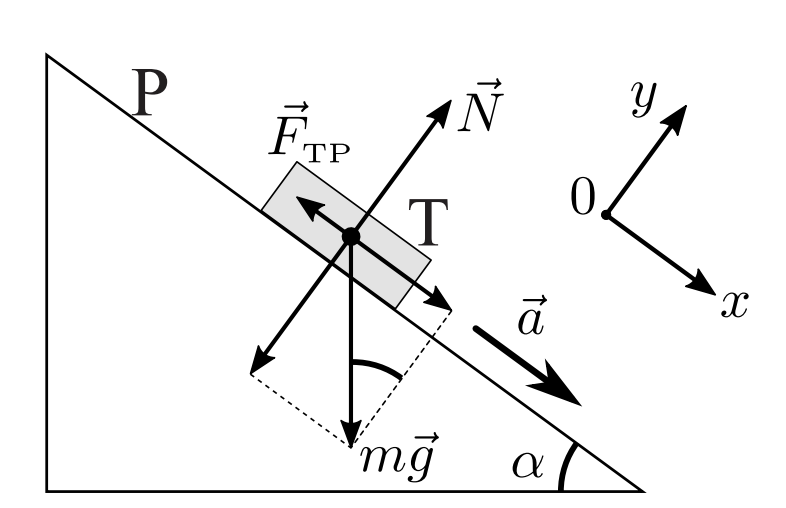
\includegraphics[width=7cm]{forces.png}
\captionof*{figure}{Схема сил, действующих на тележку}
\end{center}
%======================== 7 ========================
\punkt{7. Схема установки \textit{(перечень схем, которые составляют Приложение 1)}.}
\begin{center}
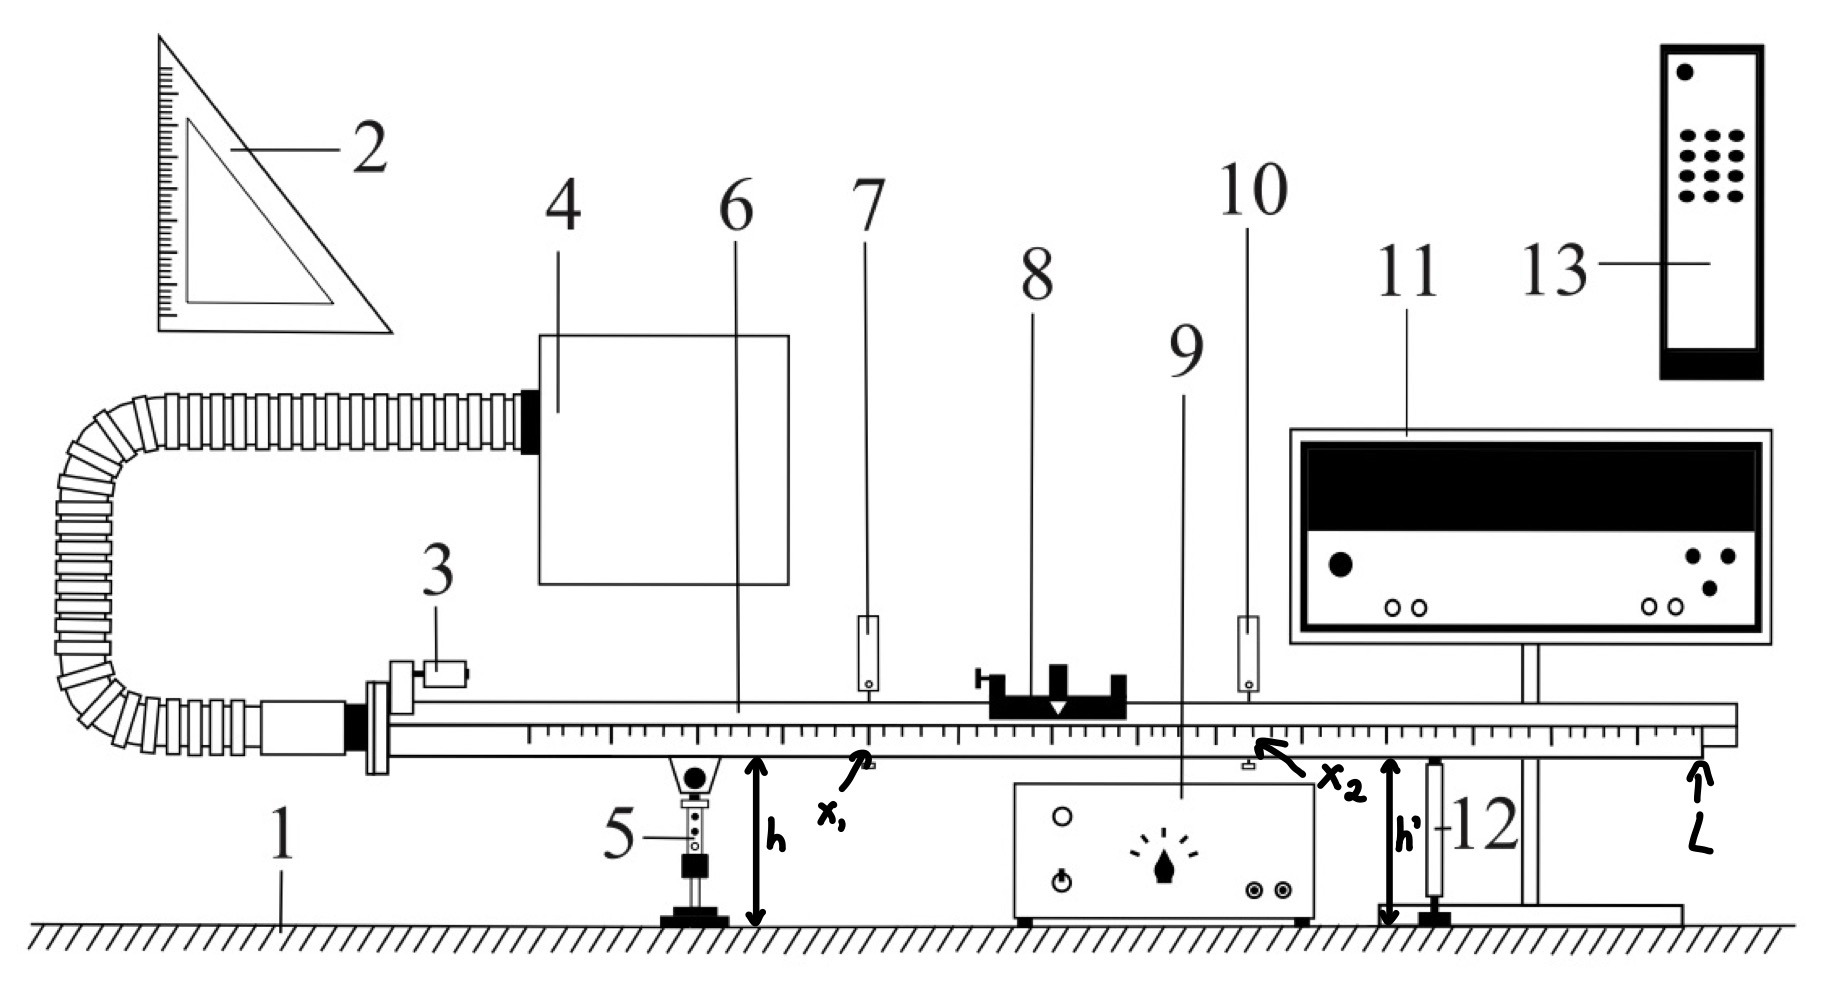
\includegraphics[width=14cm]{experimental_device.JPG}
\captionof*{figure}{Общий вид экспериментального стенда}
\end{center}

\begin{tabular}{@{}p{8cm}p{8.6cm}@{}}
1. Опорная плоскость (поверхность стола) & 8. Тележка \\
2. Линейка – угольник & 9. Источник питания насоса \\
3. Фиксирующий электромагнит & 10. Правые оптические ворота \\
4. Воздушный насос & 11. Цифровой измерительный прибор ПКЦ-3 \\
5. Левая опора рельса & 12. Правая опора рельса \\
6. Рельс с сантиметровой шкалой & 13. Пульт дистанционного управления ПКЦ-3 \\
7. Левые оптические ворота & \\
\end{tabular}

%======================== 8 ========================
\punkt{6-8. Измерительные приборы. Результаты прямых измерений и их обработки}

\begin{center}
\begin{minipage}{\linewidth}\centering

\end{minipage}\end{center}
\renewcommand{\arraystretch}{1.25}
%======================== 9 ========================
\punkt{9. Расчет результатов косвенных измерений \textit{(таблицы, примеры расчетов)}.}
\begin{center}
\begin{minipage}{\linewidth}\centering
Таблица 1 – Расчетные величины для задания 1\\[3pt]
\begin{tabular}{|C{1.0cm}|C{2.0cm}|C{2.0cm}|C{2.0cm}|C{2.0cm}|C{2.0cm}|C{2.0cm}|}
\hline
№ & $Y$, м & $\Delta_Y$, м & $\delta_Y$, \% & $Z$, с$^2$ & $\Delta_Z$, с$^2$ & $\delta_Z$, \% \\ \hline
1 & 0{,}250 & 0{,}014 & 5{,}7 & 2{,}66 & 0{,}29 & 10{,}8 \\ \hline
2 & 0{,}350 & 0{,}014 & 4{,}0 & 3{,}49 & 0{,}31 & 9{,}0 \\ \hline
3 & 0{,}550 & 0{,}014 & 2{,}6 & 5{,}41 & 0{,}37 & 6{,}8 \\ \hline
4 & 0{,}750 & 0{,}014 & 1{,}9 & 7{,}28 & 0{,}42 & 5{,}7 \\ \hline
5 & 0{,}950 & 0{,}014 & 1{,}5 & 8{,}10 & 0{,}44 & 5{,}4 \\ \hline
\end{tabular}
\end{minipage}
\end{center}

Приведем пример расчета первой строки таблицы 1.

По формуле (3) найдем $Y$ и $Z$:
\[
Y = 0{,}40 - 0{,}15 = 0{,}25\ \text{м}, \qquad
Z = \frac{2{,}6^2 - 1{,}2^2}{2} = \frac{6{,}76 - 1{,}44}{2} = 2{,}66\ \text{с}^2.
\]
Используя метод МНК(формулы 8-9), найдем коэффициент линейной зависимости $Y = aZ$ перемещения тележки $Y = x_2 - x_1$ от полуразности квадратов времени $Z = \dfrac{t_2^2 - t_1^2}{2}$, $a$ - ускорение тележки:

\begin{gather*}
\sum_{i=1}^{5} Z_iY_i = 18{,}013\ \text{м}\cdot\text{с}^2, \qquad   
\sum_{i=1}^{5} Z_i^2 = 167{,}04\ \text{с}^4,\\
a = \frac{18{,}013}{167{,}04} = 0{,}1078\ \text{м/с}^2.
\end{gather*}

\begin{center}
\begin{minipage}{\linewidth}\centering
\renewcommand{\arraystretch}{1.12}
Таблица 2 – Расчетные величины для задания 2\\[3pt]
\setlength{\tabcolsep}{2.5pt}\begin{tabular}{|C{0.9cm}|C{1.32cm}|C{1.32cm}|C{1.32cm}|C{1.32cm}|C{1.32cm}|C{1.32cm}|C{1.32cm}|C{1.32cm}|C{1.32cm}|C{1.32cm}|}
\hline
$N_\text{пл}$ & $\sin\alpha$ & $\langle t_1\rangle$, с & $\Delta_{\langle t_1\rangle}$, с & $\delta_{\langle t_1\rangle}$, \% & $\langle t_2\rangle$, с & $\Delta_{\langle t_2\rangle}$, с & $\delta_{\langle t_2\rangle}$, \% & $\langle a\rangle$, $\frac{\text{м}}{\text{с}^2}$ & $\Delta_{\langle a\rangle}$, $\frac{\text{м}}{\text{с}^2}$ & $\delta_{\langle a\rangle}$, \% \\ \hline
1 & 0{,}0128 & 1{,}20 & 0{,}067 & 5{,}6 & 4{,}30 & 0{,}110 & 2{,}6 & 0{,}111 & 0{,}007 & 5{,}8 \\ \hline
2 & 0{,}0256 & 0{,}84 & 0{,}095 & 11{,}3 & 3{,}00 & 0{,}067 & 2{,}2 & 0{,}229 & 0{,}012 & 5{,}4 \\ \hline
3 & 0{,}0359 & 0{,}76 & 0{,}095 & 12{,}5 & 2{,}42 & 0{,}087 & 3{,}6 & 0{,}360 & 0{,}031 & 8{,}5 \\ \hline
4 & 0{,}0462 & 0{,}62 & 0{,}087 & 14{,}0 & 2{,}14 & 0{,}095 & 4{,}5 & 0{,}453 & 0{,}046 & 10{,}2 \\ \hline
5 & 0{,}0590 & 0{,}50 & 0{,}067 & 13{,}3 & 1{,}90 & 0{,}067 & 3{,}5 & 0{,}565 & 0{,}045 & 7{,}9 \\ \hline
\end{tabular}
\end{minipage}
\end{center}
Приведем пример расчета для первой строки таблицы 2

По формуле (12) найдем синус угла наклона:
\[
\sin\alpha_1 = \left|\frac{(0{,}181 - 0{,}191) - (0{,}183 - 0{,}183)}{1{,}00 - 0{,}22}\right| = \frac{0{,}010}{0{,}78} = 0{,}01282.
\]

По формуле (13) найдем средние значения времени:
\[
\langle t_1\rangle = \frac{1{,}2 + 1{,}2 + 1{,}2 + 1{,}2 + 1{,}2}{5} = 1{,}2\ \text{с}, \qquad
\langle t_2\rangle = \frac{4{,}3 + 4{,}2 + 4{,}3 + 4{,}3 + 4{,}4}{5} = 4{,}3\ \text{с}.
\]

По формуле (18) найдем среднее ускорение для $N_\text{пл} = 1$ ($\langle t_1\rangle = 1{,}2$~с, $\langle t_2\rangle = 4{,}3$~с):
\[
\langle a\rangle_1 = \frac{2\,(1{,}10 - 0{,}15)}{4{,}3^2 - 1{,}2^2} = \frac{1{,}9}{18{,}49 - 1{,}44} = \frac{1{,}9}{17{,}05} = 0{,}1114\ \text{м/с}^2.
\]

Используя МНК и формулы (21), (22), найдем коэффициенты линейной зависимости $a = A + B\sin\alpha$, где $B \equiv g$ — ускорение свободного падения, $A = -F_\text{тр}/m$:
\begin{gather*}
\sum_{i=1}^{5} a_i\sin\alpha_i = 0{,}07447\ \text{м/с}^2, \qquad
\sum_{i=1}^{5} a_i = 1{,}7188\ \text{м/с}^2,\\
\sum_{i=1}^{5}\sin\alpha_i = 0{,}1795, \qquad
\sum_{i=1}^{5}\sin^2\alpha_i = 0{,}007719,
\end{gather*}
\begin{gather*}
0{,}07447 - \frac{1}{5}\cdot 1{,}7188\cdot 0{,}1795 = 0{,}01277,\\
0{,}007719 - \frac{1}{5}\cdot 0{,}1795^2 = 0{,}001275,\\
g = B = \frac{0{,}01277}{0{,}001275} = 10{,}01\ \text{м/с}^2,\\
B\sum_{i=1}^{5}\sin\alpha_i = 10{,}01\cdot 0{,}1795 = 1{,}797\ \text{м/с}^2,\\
A = \frac{1}{5}\left(1{,}719 - 1{,}797\right) = -0{,}0157\ \text{м/с}^2.
\end{gather*}

%======================== 10 ========================
\punkt{10. Расчет погрешностей измерений \textit{(для прямых и косвенных измерений)}.}

Рассчитаем погрешности для первой строки таблицы 1. По формулам (4), (5):
\begin{gather*}
\Delta_Y = \sqrt{2}\cdot 0{,}01 = 0{,}0141\ \text{м},\\
\delta_{Y_1} = \frac{0{,}0141}{0{,}25}\cdot 100\,\% = 5{,}7\,\%.
\end{gather*}
По формулам (6), (7):
\begin{gather*}
\Delta_{Z_1} = 0{,}1\cdot\sqrt{1{,}2^2 + 2{,}6^2} = 0{,}1\cdot\sqrt{8{,}2} = 0{,}286\ \text{с}^2,\\
\delta_{Z_1} = \frac{0{,}286}{2{,}66}\cdot 100\,\% = 10{,}8\,\%.
\end{gather*}

Рассчитаем погрешность ускорения тележки, найденного МНК. Отклонения точек от прямой $Y = aZ$:
\begin{align*}
Y_1-aZ_1 &= 0{,}25 - 0{,}1078\cdot2{,}66 = -0{,}0368\\
Y_2-aZ_2 &= 0{,}35 - 0{,}1078\cdot3{,}485 = -0{,}0258\\
Y_3-aZ_3 &= 0{,}55 - 0{,}1078\cdot5{,}405 = -0{,}0328\\
Y_4-aZ_4 &= 0{,}75 - 0{,}1078\cdot7{,}28 = -0{,}0350\\
Y_5-aZ_5 &= 0{,}95 - 0{,}1078\cdot8{,}1 = 0{,}0766
\end{align*}
\[
\sum_{i=1}^{5}\left(Y_i - aZ_i\right)^2 = 0{,}01019\ \text{м}^2.
\]
По формуле (9) найдем СКО:
\[
S_a = \sqrt{\frac{0{,}01019}{(5-1)\cdot 167{,}04}} = 0{,}00391\ \text{м/с}^2.
\]
По формулам (10), (11):
\begin{gather*}
\Delta_a = 2\cdot 0{,}00391 = 0{,}0078\ \text{м/с}^2,\\
\delta_a = \frac{0{,}0078}{0{,}1078}\cdot 100\,\% = 7{,}2\,\%.
\end{gather*}

Рассчитаем погрешности для первой строки таблицы 2 ($N_\text{пл} = 1$)

По формуле (14) вычислим оценку СКО:
\begin{gather*}
\sum_{i=1}^{5}\left(t_{1i} - \langle t_1\rangle\right)^2 = 0\ \text{с}^2, \qquad 
S_{\langle t_1\rangle} = \sqrt{\frac{0}{5\cdot 4}} = 0\ \text{с},\\[4pt]
\sum_{i=1}^{5}\left(t_{2i} - \langle t_2\rangle\right)^2 = 0{,}02\ \text{с}^2,\qquad
S_{\langle t_2\rangle} = \sqrt{\frac{0{,}02}{5\cdot 4}} = 0{,}0316\ \text{с}.
\end{gather*}
Рассчитаем величину случайной погрешности по формуле (15), коэффициент Стьюдента $t_{0{,}95;\,5} = 2{,}78$:
\[
\Delta_{\langle t_1\rangle} = 2{,}78\cdot 0 = 0\ \text{с}, \qquad
\Delta_{\langle t_2\rangle} = 2{,}78\cdot 0{,}0316 = 0{,}0879\ \text{с}.
\]
Вычислим абсолютную погрешность измерения времени по формуле (16) с учетом случайной и инструментальной погрешности ($\Delta_\text{и} = 0{,}1$~с):
\begin{gather*}
\Delta_{t_1} = \sqrt{0^2 + \left(\tfrac{2}{3}\cdot 0{,}1\right)^2} = 0{,}0667\ \text{с},\\
\Delta_{t_2} = \sqrt{0{,}0879^2 + \left(\tfrac{2}{3}\cdot 0{,}1\right)^2} = 0{,}110\ \text{с}.
\end{gather*}
Определим относительную погрешность измерения времени по формуле (17):
\[
\delta_{t_1} = \frac{0{,}0667}{1{,}2}\cdot 100\,\% = 5{,}6\,\%, \qquad
\delta_{t_2} = \frac{0{,}110}{4{,}3}\cdot 100\,\% = 2{,}6\,\%.
\]

Погрешность ускорения для $N_\text{пл} = 1$ по формуле (19) ($\Delta_{x_{\text{и}1}} = \Delta_{x_{\text{и}2}} = 0{,}01$~м):
\begin{gather*}
\frac{0{,}01^2 + 0{,}01^2}{(1{,}10 - 0{,}15)^2} = 0{,}00022,\\
\left(1{,}2\cdot 0{,}0667\right)^2 = 0{,}0064, \qquad
\left(4{,}3\cdot 0{,}110\right)^2 = 0{,}225,\\
4\cdot\frac{0{,}0064 + 0{,}225}{17{,}05^2} = 0{,}00319,
\end{gather*}
\[
\Delta_{\langle a\rangle_1} = 0{,}1114\cdot\sqrt{0{,}00022 + 0{,}00319} = 0{,}0065\ \text{м/с}^2.
\]
По формуле (20):
\[
\delta_{\langle a\rangle_1} = \frac{0{,}0065}{0{,}1114}\cdot 100\,\% = 5{,}8\,\%.
\]

Используя формулы (23)–(27), найдем погрешность ускорения свободного падения:
{\small\begin{align*}
d_1 &= 0{,}1114 - \left(-0{,}0157 + 10{,}01\cdot0{,}0128\right) = -0{,}0012\\
d_2 &= 0{,}2291 - \left(-0{,}0157 + 10{,}01\cdot0{,}0256\right) = -0{,}0120\\
d_3 &= 0{,}3599 - \left(-0{,}0157 + 10{,}01\cdot0{,}0359\right) = 0{,}0162\\
d_4 &= 0{,}4529 - \left(-0{,}0157 + 10{,}01\cdot0{,}0462\right) = 0{,}0064\\
d_5 &= 0{,}5655 - \left(-0{,}0157 + 10{,}01\cdot0{,}0590\right) = -0{,}0094
\end{align*}}
\[
\sum_{i=1}^{5} d_i^2 = 0{,}000536, \qquad
D = 0{,}007719 - \frac{1}{5}\cdot 0{,}1795^2 = 0{,}001275,
\]
\[
S_g = \sqrt{\frac{0{,}000536}{0{,}001275\cdot(5-2)}} = 0{,}374\ \text{м/с}^2,
\]
\begin{gather*}
\Delta_g = 2\cdot 0{,}374 = 0{,}75\ \text{м/с}^2,\\
\delta_g = \frac{0{,}75}{10{,}01}\cdot 100\,\% = 7{,}5\,\%.
\end{gather*}
Отклонение экспериментального значения от табличного $g_\text{табл} = 9{,}82$~м/с$^2$ по формуле (28):
\begin{gather*}
\Delta g_\text{откл} = \left|10{,}01 - 9{,}82\right| = 0{,}19\ \text{м/с}^2,\\
\delta g_\text{откл} = \frac{0{,}19}{9{,}82}\cdot 100\,\% = 2{,}0\,\%.
\end{gather*}
%======================== 11 ========================
\punkt{11. Графики \textit{(перечень графиков, которые составляют Приложение 2)}.}
\begin{minipage}{\linewidth}
График линейной зависимости между перемещением и полуразностью квадратов значений времени \(x_2 - x_1 = \frac{a}{2} \left( t_2^2 - t_1^2 \right)\), и соответствующие экспериментальные точки: \\

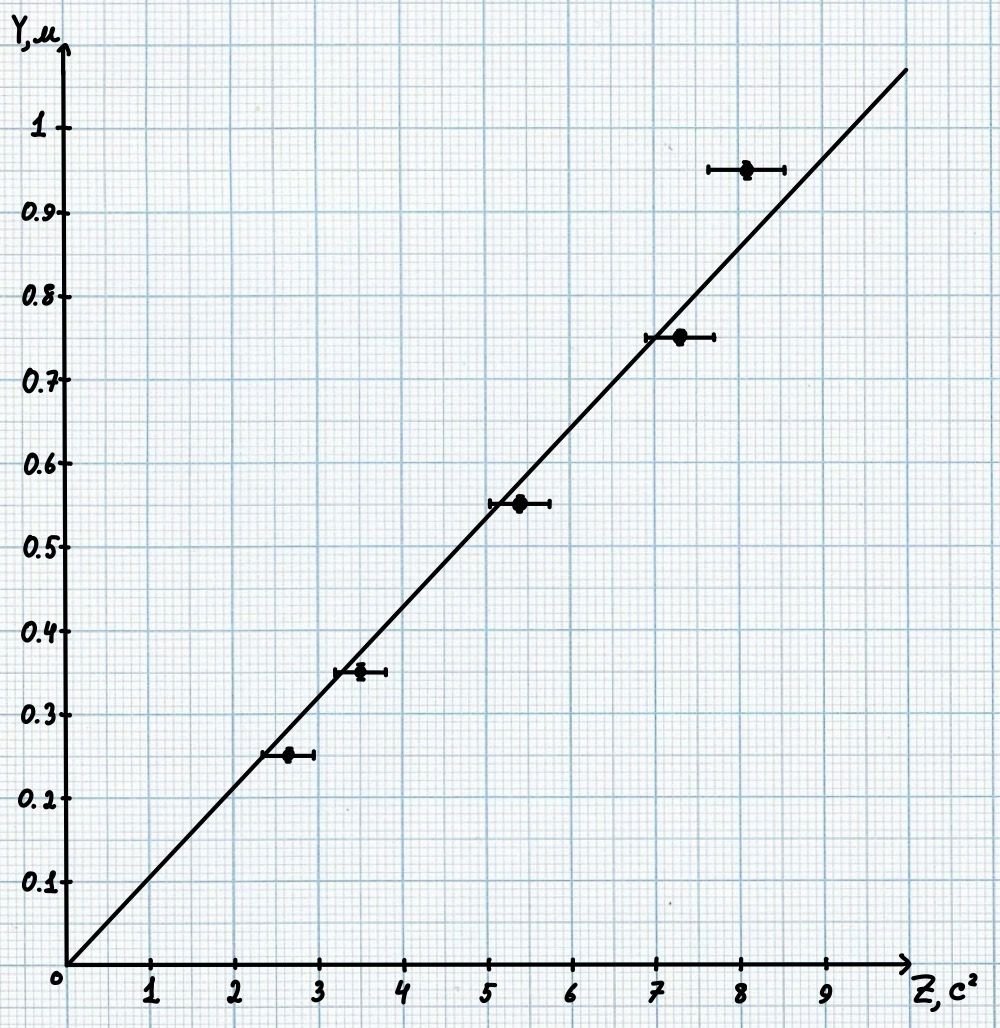
\includegraphics[width=14cm]{first.JPG}
\\
\end{minipage}
\begin{minipage}{\linewidth}
График аппроксимирующей линейной зависимости $a = A + B\sin\alpha$, и соответствующие экспериментальные точки: \\
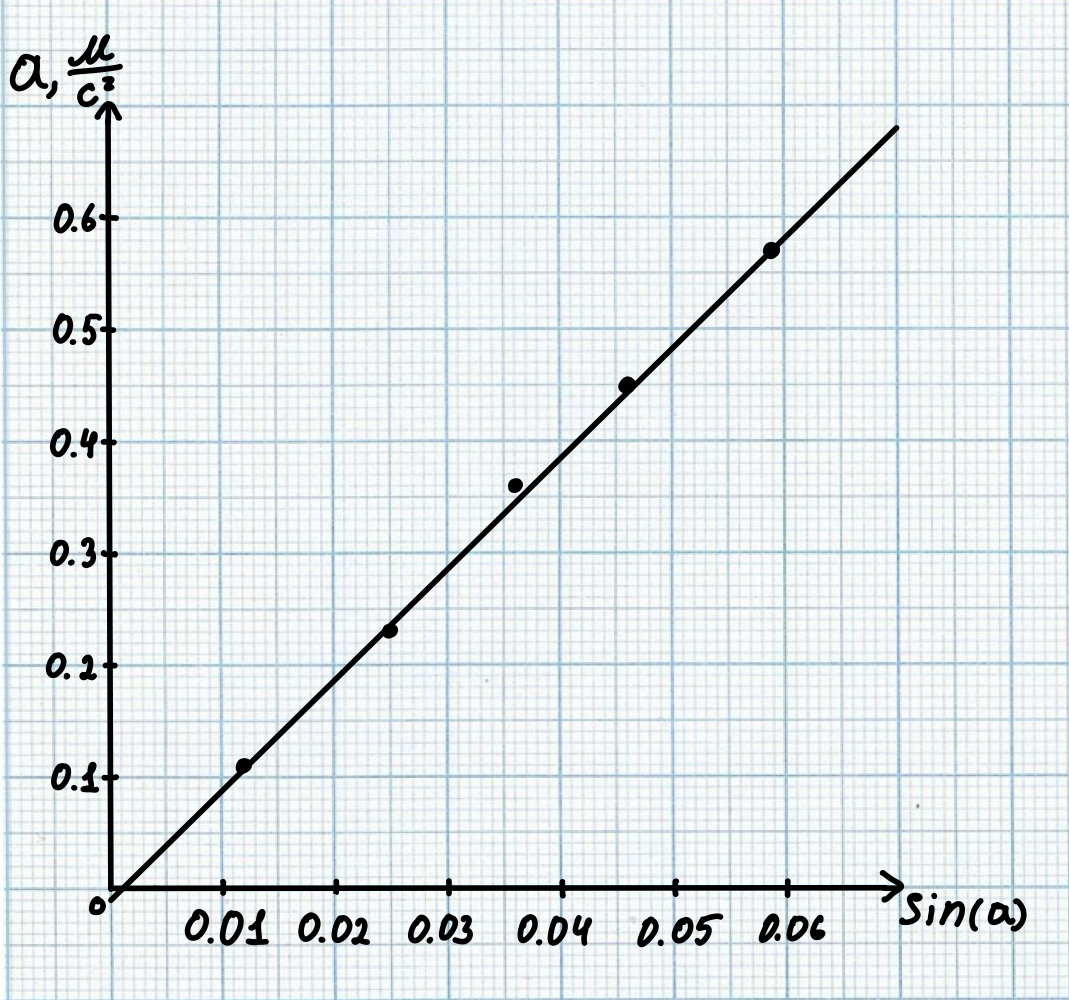
\includegraphics[width=14cm]{second.jpeg}
\end{minipage}
%======================== 12 ========================
\punkt{12. Окончательные результаты.}
Задание 1:
\begin{itemize}
  \item $a = (0{,}108 \pm 0{,}008)$ м/с$^2$; \quad $\delta_a = 7{,}2\,\%$; \quad $P = 0{,}95$.
\end{itemize}
Задание 2:
\begin{itemize}
  \item $g = (10{,}01 \pm 0{,}75)$ м/с$^2$; \quad $\delta_g = 7{,}5\,\%$; \quad $P = 0{,}95$.
  \item $A = -F_\text{тр}/m = -0{,}016$ м/с$^2$.
\end{itemize}
Отклонение от табличного значения $g_\text{табл} = 9{,}82$ м/с$^2$:
\begin{itemize}
  \item $\Delta g_\text{откл} = 0{,}19$ м/с$^2$; \quad $\delta g_\text{откл} = 2{,}0\,\%$.
\end{itemize}
Интервальная оценка:
\begin{itemize}
  \item Доверительный интервал ускорения тележки: $0{,}100 \le a \le 0{,}116$ м/с$^2$.
  \item Доверительный интервал ускорения свободного падения: $9{,}27 \le g \le 10{,}76$ м/с$^2$; табличное значение $g_\text{табл} = 9{,}82$ м/с$^2$ находится в пределах этого интервала.
\end{itemize}
\clearpage
%======================== 13 ========================
\punkt{13. Выводы и анализ результатов работы.}
Анализ зависимости $Y = f(Z)$:
\begin{itemize}
  \item Экспериментальные точки ложатся вблизи прямой, проходящей через начало координат, что подтверждает линейную зависимость перемещения от полуразности квадратов времени и, следовательно, равноускоренный характер движения тележки.
\end{itemize}
Анализ зависимости $a = f(\sin\alpha)$:
\begin{itemize}
  \item Среднее ускорение тележки растёт с увеличением угла наклона рельса, экспериментальные точки в пределах погрешностей ложатся на прямую $a = A + B\sin\alpha$.
  \item Ускорение свободного падения, определённое по угловому коэффициенту, $g = (10{,}01 \pm 0{,}75)$ м/с$^2$; табличное значение $9{,}82$ м/с$^2$ попадает в доверительный интервал, отклонение составляет $0{,}19$ м/с$^2$.
  \item Свободный член $A = -0{,}016$ м/с$^2$ отрицателен, что соответствует наличию малой силы трения: $F_\text{тр}/m \approx 0{,}016$ м/с$^2$.
\end{itemize}
Основной вклад в погрешности вносит инструментальная точность секундомера. Для повышения точности следует регистрировать время с большим числом знаков и увеличить число измерений.

%======================== 14–16 ========================
\punkt{14. Дополнительные задания.}
\vspace{2cm}
\punkt{15. Выполнение дополнительных заданий.}
\vspace{2cm}
\punkt{16. Замечания преподавателя \textit{(исправления, вызванные замечаниями преподавателя, также помещают в этот пункт)}.}
\vspace{5cm}

\begin{tabular}{@{}p{2.6cm}p{13.5cm}@{}}
\textbf{\textit{\small Примечание:}} &
\parbox[t]{13.5cm}{\small\itshape
1. Пункты 1-6,8-13 Протокола-отчета \textbf{обязательны} для заполнения.\\
2. Необходимые исправления выполняют непосредственно в протоколе-отчете.\\
3. При ручном построении графиков рекомендуется использовать миллиметровую бумагу.\\
4. Приложения 1 и 2 вкладывают в бланк протокола-отчета.}
\end{tabular}

\end{document}x